\section{Distributing Work}

Simulating thousands of agents and millions of grid cells simultaneously at a reasonable speed will require multiple machines. One process, the \emph{game master}, is responsible for starting the game and reporting the rules. $n_ac$ more processes, on the same machine or another, act as \emph{agent coordinators} responsible for launching and communicating with agent processes. They are responsible for delivering messages, taking and executing agent orders, and reporting success or failure. Coordinators communicate between themselves over persistent TCP connections.

Agents interact in two primary ways: messages and movement. Both are only effective within a certain proximity of the agent. These properties suggest that agents should be assigned to coordinators based on proximity, perhaps running as processes on the same server as their agent coordinator. There are multiple ways to perform this assignment. This paper considers three strategies: static assignment, fixed region distribution, and dynamic grid distribution. (There is a simpler case that will not be considered, i.e. the case in which the game master acts as the only coordinator.)

\subsection{Static Assignment}

The simplest way to assign agents to coordinators is to assign $\frac{n_agents}{n_ac}$ agents to each agent coordinator at random or based on some positioning heuristic. No agents will ever change their coordinators.

This approach introduces significant overhead. Each agent coordinator will have to send all available information to all other coordinators every single turn because it cannot know which other coordinators contain agents close to its own.

\subsection{Fixed Region Distribution}

One way to alleviate the communication problem is to assign each agent coordinator a fixed portion of the grid to be responsible for. An example of such an assignment is shown in figure \ref{fixed}. There will never be a recalculation of coordinator bounds and each coordinator has a constant set of neighbor coordinators to communicate with. Each turn, adjacent coordinators exchange messages, order confirmations for agents near their shared border, and full agent information transfers for agents moving from one coordinator's region to a neighbor's region.

\begin{figure*}
    \begin{center}
        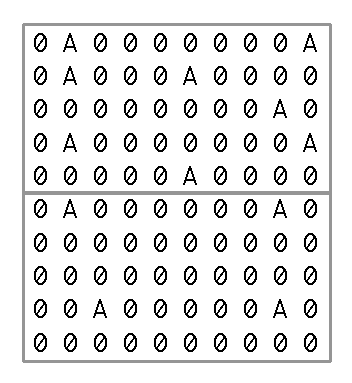
\includegraphics[scale=0.5]{figures/assign_region.pdf}
    \end{center}
    \caption{Region split across two coordinators. The top coordinator has 8 agents and the bottom coordinator has 4.}
    \label{fixed}
\end{figure*}

This strategy requires the least communication between agent coordinators when agents move relatively little, but requires much communication when many agents are near region borders or move between borders often. It also introduces inefficiency in work distribution when disproportionate numbers of agents are gathered in small regions.

\subsection{Dynamic Grid Distribution}

Like fixed region distribution, dynamic grid distribution assigns each agent coordinator a region of the grid to be responsible for. However, the regions can be resized while the simulation is running, partially alleviating the work distribution problem, making sure that every coordinator controls approximately the same number of agents as the rest. Figure \ref{dynamic} shows region assignments for two coordinators during a run.

\begin{figure*}
    \begin{center}
        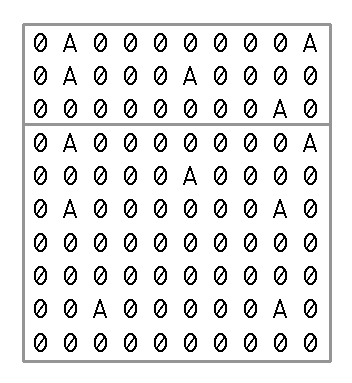
\includegraphics[scale=0.5]{figures/assign_split.pdf}
    \end{center}
    \caption{Fair agent split across two coordinators. Both coordinators have 6 agents.}
    \label{dynamic}
\end{figure*}

\subsection{This Version}

The initial implementation of Tecellate uses static assignment based on rectangular regions to test communication protocols and basic mechanics. 
